\chapter{Experimentelle Resultate und Analysen}
\label{chapter:experiment}

Im Folgenden sollen die im Rahmen dieser Arbeit aufgenommenen Daten vorgestellt und ausgewertet werden. Dabei lassen sich zwei separate Bemühungen unterscheiden. Zum einen wurden Untersuchungen zur Dynamik in CRN angestellt, welche zuerst präsentiert werden sollen, zum anderen wurden die Linienformänderungen in Abhängigkeit der Temperatur untersucht und mit theoretischen Überlegungen verglichen.

Im Verlauf der Auswertung werden die Daten zum Teil nach dem verwendeten Spektrometer unterschieden. Dies liegt an der unterschiedlichen Larmorfrequenzen der Apparaturen -- $\omega_{L, \text{OBI}} / 2\pi = f_{L, \text{OBI}} = \SI{97.1722}{MHz}$ im Vergleich zu $\omega_{L, \text{Bruker}} / 2\pi = f_{L, \text{Bruker}} = \SI{130.9736}{MHz}$ -- welche sich um etwa einen Faktor $\SI{1.35}{}$ unterscheiden. Dies ist genug, um eine deutliche Auswirkung in den Daten beobachten zu können.

Bei beiden Spektrometern wurden für die grundlegenden Parameter bei allen Messungen etwa die gleichen Einstellungen verwendet: Für das OBI-Spektrometer wurde die Dauer eines $\SI{180}{\degree}$-Pulses auf einen Wert zwischen $\SI{6.5}{\micro s}$ und $\SI{7.1}{\micro s}$ gesetzt, beim Bruker-Spektrometer auf $\SI{5.2}{\micro s}$. Dabei wurde selektiv die Zentrallinie angeregt. Das bedeutet, dass das $^\text{87}$Rb-NMR-Spektrum zu breit ist, als dass es nicht-selektiv angeregt werden könnte, und da es sich bei $^\text{87}$Rb um einen Kern mit halb-zahligen Spin handelt, wird nur der Übergang $-\sfrac{1}{2} \leftrightarrow \sfrac{1}{2}$ -- welcher im Spektrum als sogenannte Zentrallinie zu sehen ist -- angeregt.

Die Evolutionszeit $t_p$ der Echos beträgt in den meisten Fällen $\SI{15}{\micro s}$ und nie mehr als $\SI{20}{\micro s}$. Die Wiederholungszeit, also die Zeit zwischen zwei Pulsfolgen, beträgt zwischen $\SI{10}{\milli s}$ und $\SI{50}{\milli s}$. Dies soll dafür sorgen, dass die Magnetisierung nach jeder Pulsfolge wieder in den Ausgangszustand jeder Pulsfolge, der Gleichgewichtsmagnetisierung, zurückkehren kann. Dafür sollte ein Vielfaches der $T_1$-Zeitkonstante gewartet werden.

Der mit dem OBI-Spektrometer abgedeckte Temperaturbereich reicht von $\SI{230}{\kelvin}$ bis $\SI{435}{\kelvin}$, während sich der Temperaturbereich des Bruker-Spektrometers auf den Bereich von $\SI{310}{\kelvin}$ bis $\SI{390}{\kelvin}$ beschränkt.

Alle beschriebenen Fits wurden durch eine least-squares-Methode mit Hilfe von Python-Skripten, welche \texttt{scipy.optimize}- oder \texttt{lmfit}-Routinen verwenden, erstellt.


\section{Bestimmung von $T_1$ und $T_2$} \label{section:res:T_1}

Vor dem Beginn jeder NMR-Messung ist es sinnvoll, $T_1$, die Zeitkonstante der longitudinalen Relaxation, im zu untersuchenden Temperaturgebiet zu vermessen. Dies ist hilfreich, um wichtige Parameter der Messungen abzustecken und mögliche Hindernisse im Vorhinein abschätzen zu können. So sollte zwischen allen Messungen eine Zeit von mindestens $4 T_1$ gewartet werden um sicherzugehen, dass sich die Magnetisierung in guter Näherung wieder im Gleichgewichtszustand befindet -- wird $T_1$ also im Laufe der Messung bei anderen Temperaturen länger, muss hierauf Rücksicht genommen werden. Wird $T_1$ auf der anderen Seite sehr kurz, kehrt die Magnetisierung sehr schnell in den Gleichgewichtszustand zurück und lassen dem Experimentierenden daher nur ein kleines Fenster, in dem Untersuchungen durchgeführt werden können. Hinzu kommt, dass der Temperaturverlauf von $T_1$ nach Formel \eqref{eqn:bpp} wertvolle Information über die Dynamik in der untersuchten Probe liefern kann. Zuletzt bietet diese recht einfache und reproduzierbare Messung die Möglichkeit, das Spektrometer und die Probe auf Übereinstimmung mit Literaturdaten hin zu überprüfen. Daher wurden zu allen untersuchten Temperaturen $T_1$-Messungen aufgenommen.

Zur Bestimmung von $T_1$ wurde eine Invertierungs-Pulsfolge mit Hahn-Echo verwendet. Repräsentative Rohdaten einer solchen Messung sind in Abbildung \ref{fig:res:T_1_roh} zu sehen. An die Daten wurden Fits mit $T_1$ und $\beta$ als freien Parametern entsprechend Gleichung \eqref{eqn:theo:T_1_fit} angelegt -- diese sind als Linien dargestellt. Die Daten wurden hier zudem mit $M_{T_1}(0) = -1$ und $M_{T_1}(\infty) = 1$ normiert, um einen besseren Vergleich zuzulassen. Es ist zu erkennen, dass die Fits eine gute Repräsentation der Daten ermöglichen.
\begin{figure}
	\begin{center}
		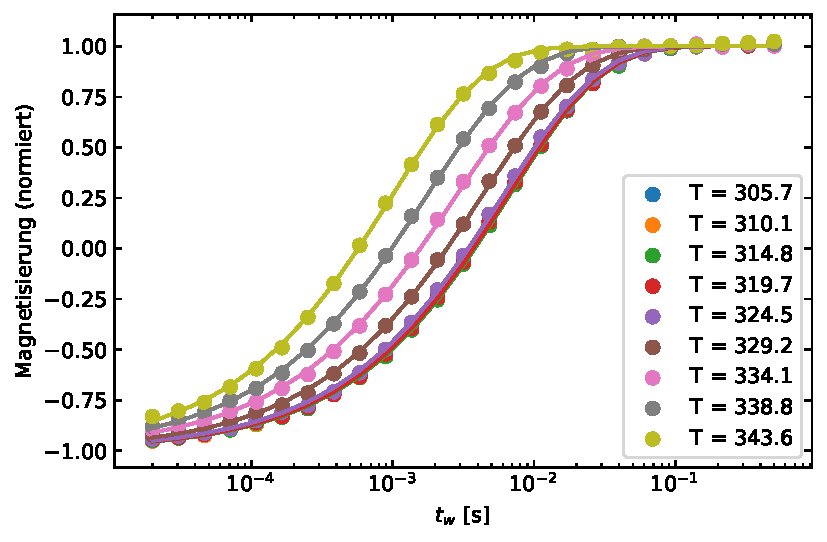
\includegraphics[width=.8\textwidth]{graphics/plot/t1_roh3.pdf}
	\end{center}
	\caption{Aufbaukurven der longitudinalen Magnetisierung zur Bestimmung von $T_1$, aufgenommen am OBI-Spektrometer mit $\omega_{L, \text{OBI}} = 2\pi \cdot \SI{97.1722}{MHz}$. Linien stellen Kohlrausch-Fits an die Datenpunkte dar. Die Daten wurden mit $M_{T_1}(0) = -1$ und $M_{T_1}(\infty) = 1$ der Fits normiert.} \label{fig:res:T_1_roh}
\end{figure}

Während sich die Kurven zwischen $\SI{305}{\kelvin}$ und $\SI{325}{\kelvin}$ sehr ähneln, verschieben sich die Kurven und damit auch die $T_1$-Werte bei höheren Temperaturen zu kürzeren Zeiten.

Dies lässt sich auch in der Gesamtübersicht aller aufgenommenen $T_1$-Daten in Abbildung \ref{fig:res:T_1} erkennen. Während die $T_1$-Zeiten bei Temperaturen von $\SI{250}{\kelvin}$ bis $\SI{325}{\kelvin}$ nahezu unverändert im unteren Millisekunden-Bereich liegen, verkürzen sie sich bei steigenden Temperaturen bis in den zweistelligen Mikrosekunden-Bereich. Es ist ein $T_1$-Minimum bei etwa $\SI{410}{\kelvin}$ mit einem Wert von ungefähr $\SI{5}{\micro s}$ auszumachen, ehe die $T_1$-Zeiten wieder länger werden.
\begin{figure}
	\begin{center}
		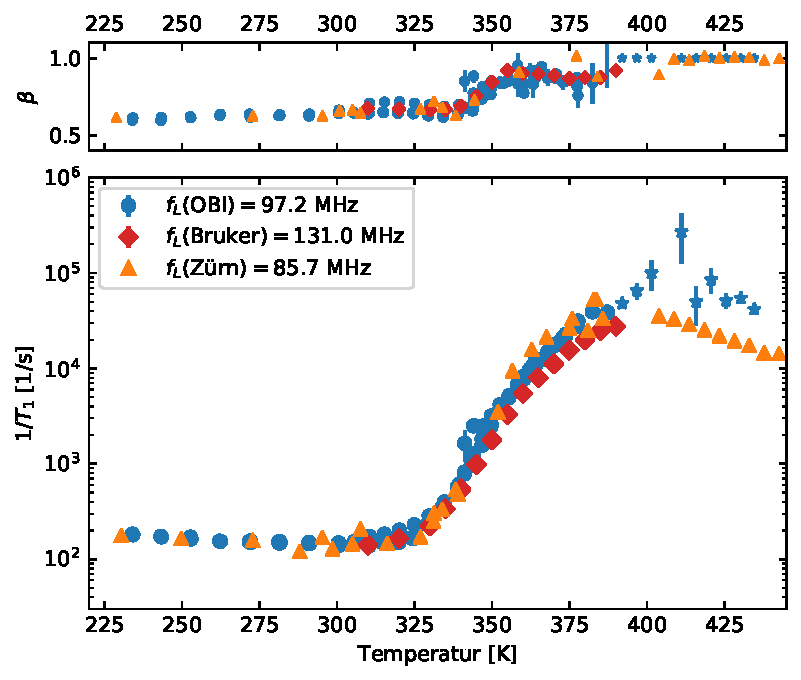
\includegraphics[width=\textwidth]{graphics/plot/t1.pdf}
	\end{center}
	\caption{$T_1$ und $\beta$ aus Fits nach Gleichung \eqref{eqn:theo:T_1_fit}. Blaue und rote Symbole zeigen die am OBI- bzw. Bruker-Spektrometer aufgenommen Daten. Bei Temperaturen über $\SI{390}{\kelvin}$ wurden die $\beta$ der Fits auf $\SI{1}{}$ festgesetzt -- diese Werte wurden mit Sternen anstatt Punkten symbolisiert. Orangene Dreiecke bieten einen Vergleich mit Daten von Zürn \cite{zuern_paper}.} \label{fig:res:T_1}
\end{figure}

Während die Unsicherheiten der Fits die Größe der dargestellten Symbole meist nicht überschreiten, sind größere Schwankungen über $\SI{390}{\kelvin}$ zu erkennen. Daher wurde hier bei den Fits konstant $\beta = 1$ gesetzt -- symbolisiert durch Sterne anstatt Punkte --, um diese Schwankungen möglichst gering zu halten.

Abgesehen von dem erwähnten Temperaturbereich ist eine gute Übereinstimmung des Verlaufs der $T_1$-Daten von Zürn \cite{zuern_paper}, welche an einem Spektrometer mit einer Larmorfrequenz von $\omega_{L, \text{Zürn}} = 2\pi \cdot \SI{85.7}{MHz}$ aufgenommen wurden, zu erkennen. Die vorhandenen Differenzen könnten durch die unterschiedlichen Larmorfrequenzen der Aufbauten verursacht worden sein. Zudem sind kaum Differenzen zwischen Messungen des OBI-Spektrometers mit überlappenden Temperaturbereichen, wie sie zwischen $\SI{330}{\kelvin}$ und $\SI{370}{\kelvin}$ auftreten, zu erkennen. Dies lässt darauf schließen, dass diese Daten gut reproduzierbar sind.

Die am Bruker-Spektrometer mit $\omega_{L, \text{Bruker}} = 2\pi \cdot \SI{130.9736}{MHz}$ aufgenommenen Daten folgen dem gleichen beschriebenen Verlauf und zeigen bis auf den Temperaturbereich zwischen $\SI{360}{\kelvin}$ und $\SI{390}{\kelvin}$ keinen nennenswerte Differenzen zu den Daten von Zürn oder den Daten des OBI-Spektrometers; dort aber sind die gemessenen $T_1$-Daten zu leicht längeren Zeiten verschoben. Der Quotient der $T_1$-Zeiten der beiden Spektrometer überschreitet den Wert $\SI{2}{}$ jedoch nicht.

Im oberen Teil der Abbildung \ref{fig:res:T_1} sind die entsprechenden $\beta$ der Fits zu sehen. Von einem Wert von $\SI{0.6}{}$ bei tieferen Temperaturen steigen sie zu einem Wert von etwa $\SI{0.9}{}$ bei Temperaturen über $\SI{350}{\kelvin}$. Dies entspricht etwa den Ergebnissen von Zürn. Bei Temperaturen oberhalb von $\SI{390}{\kelvin}$ wurden die $\beta$ der Fits, wie erwähnt, auf 1 festgesetzt -- wieder durch Stern-Symbole anstatt von Punkten dargestellt. Die Messunsicherheiten, die diesen Schritt notwendig machen, stammen daher, dass mit den verwendeten Apparaturen nicht verlässlich Datenpunkte vor $\SI{10}{\micro s}$ aufgenommen werden können. Wenn die $T_1$ Zeit aber in der gleichen Größenordnung liegt und zum Zeitpunkt des $T_1$-Werts das Signal auf etwa $1/e$ abgefallen ist, ist es verständlich, dass ein Fit Schwierigkeiten bereiten kann. Lösen ließe sich dies theoretisch mit einer längeren Evolutionszeit des verwendeten Echos; dies ist aufgrund der kurzen $T_1$- und $T_2$-Zeiten in diesem Temperaturbereich jedoch nicht möglich -- das entstehende Signal ist zu klein, um effektiv vom Rauschen getrennt zu werden.

Die Unsicherheiten der mit dem Bruker-Spektrometer bestimmten $\beta$ ist vergleichsweise gering -- die Fehlerbalken überschreiten die Größe der Symbole nicht. Dies ist mit der höheren Qualität der Daten (besonders auch bei den Linienformen der Spektren in Abbildung \ref{fig:res:bruker_linienform} im Vergleich zu \ref{fig:res:spek_linienform} zu erkennen) und den niedrigeren $T_1$-Werten zu erklären.



% \section{$T_2$} \label{section:res:T_2}
\par\bigskip


Ähnlich wie $T_1$ ist auch $T_2$ eine wichtige Größe, die Parameter für folgende Messungen bestimmen kann -- so werden beispielsweise die praktikablen Längen von Pulsabständen, in denen transversale Magnetisierung vorliegt, von $T_2$ begrenzt. Zudem kann nach Formel \eqref{eqn:theo:T_2_dyn} Aufschluss über Dynamiken gegeben werden.

In Abbildung \ref{fig:res:T_2_roh} sind exemplarisch Rohdaten verschiedener Temperaturen zu sehen. Diese wurden mit einem Hahn-Echo mit $\tau = \SI{15}{\micro s}$ aufgenommen und auf den Bereich zwischen $\SI{0}{}$ und $\SI{1}{}$ normiert.
\begin{figure}
	\begin{center}
		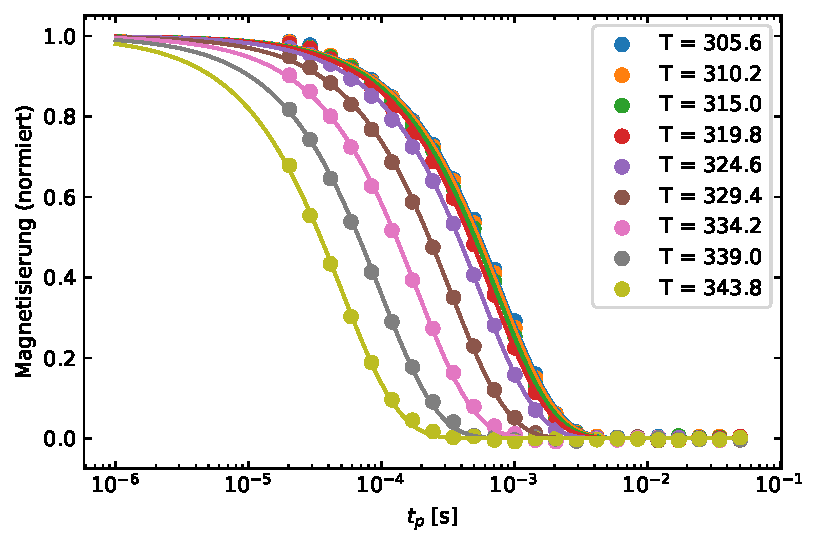
\includegraphics[width=.8\textwidth]{graphics/plot/t2_roh3.pdf}
	\end{center}
	\caption{Kurven des transversalen Magnetisierungszerfalls zur Bestimmung von $T_2$, aufgenommen am OBI-Spektrometer mit $\omega_{L, \text{OBI}} = 2\pi \cdot \SI{97.1722}{MHz}$. Linien stellen Kohlrausch-Fits an die Datenpunkte dar. Die Daten wurden auf $M_{T_2}(0) = 1$ und $M_{T_2}(\infty) = 0$ der Fits normiert.} \label{fig:res:T_2_roh}
\end{figure}
An diese wurden Fit-Funktionen nach \eqref{eqn:theo:T_2_fit} angelegt, welche als Linien dargestellt sind. Es lässt sich mit den Fits eine gute Übereinstimmung zu den Daten erzielen. Auch hier lässt sich erkennen, dass $T_2$ bei Temperaturen bis etwa $\SI{320}{\kelvin}$ nahezu konstant verbleibt und zu hoheren Temperaturen kleiner wird.

Abbildung \ref{fig:res:T_2} zeigt eine Übersicht über die aufgenommen $T_2$-Werte mit den zugehörigen $\beta$ der Fits. Unter $\SI{320}{\kelvin}$ verbleiben erstere im niedrigen Millisekunden-Bereich, ehe sie deutlich kürzer werden und sich bei etwa $\SI{360}{\kelvin}$ ein Minimum zeigt. Die Werte des Bruker-Spektrometers sind hiermit in guter Übereinstimmung, wobei wiederum festzuhalten ist, dass die Messunsicherheiten geringer sind. Ein zweites Minimum zeigt sich bei etwa $\SI{400}{\kelvin}$, dessen Wert sich, ebenso wie der erste, im zweistelligen Mikrosekunden-Bereich befindet. Zwischen $\SI{400}{\kelvin}$ und $\SI{410}{\kelvin}$ ist zu erkennen, dass -- wohl durch die Kürze von $T_2$ bei diesen Temperaturen -- deutlich größere Unsicherheiten als im Rest der Messreihe vorliegen, wo sie in guter Näherung vernachlässigbar sind.

Aus diesem Grund wurden hier zusätzliche Fits mit einem Konstanten $\beta = 1$ angefertigt, die in der Abbildung durch Sterne symbolisiert sind. Es ist zu erkennen, dass die so bestimmten $T_2$-Werte deutlich geringere Unsicherheiten zeigen, aber dem gleichen Verlauf folgen. Sie scheinen jedoch bei etwas kürzeren Werten zu liegen; der Quotient der Werte mit ihrem mit freiem $\beta$ bestimmten Gegenpart überschreitet den Wert 2 nicht.

Auch die $\beta$-Werte zeigen bei höheren Temperaturen deutlich größere Unsicherheiten, hier allerdings schon zwischen $\SI{390}{\kelvin}$ und $\SI{425}{\kelvin}$. Sie scheinen zwischen $\SI{1}{}$ und $\SI{2}{}$ zu liegen. Bei tieferen Temperaturen klärt sich das Bild etwas: Während die Daten des OBI-Spektrometers bei Temperaturen bis $\SI{350}{\kelvin}$ ein $\beta$ zwischen $\SI{1}{}$ und $\SI{1.5}{}$ suggerieren, zeigen die Daten des Bruker-Spektrometers ein $\beta$ um $\SI{1}{}$ -- mit geringerer Unsicherheit. Bei nochmals tieferen Temperaturen scheint $\beta$ konsistent bei rund $\SI{1}{}$ zu liegen.

\begin{figure}
	\begin{center}
		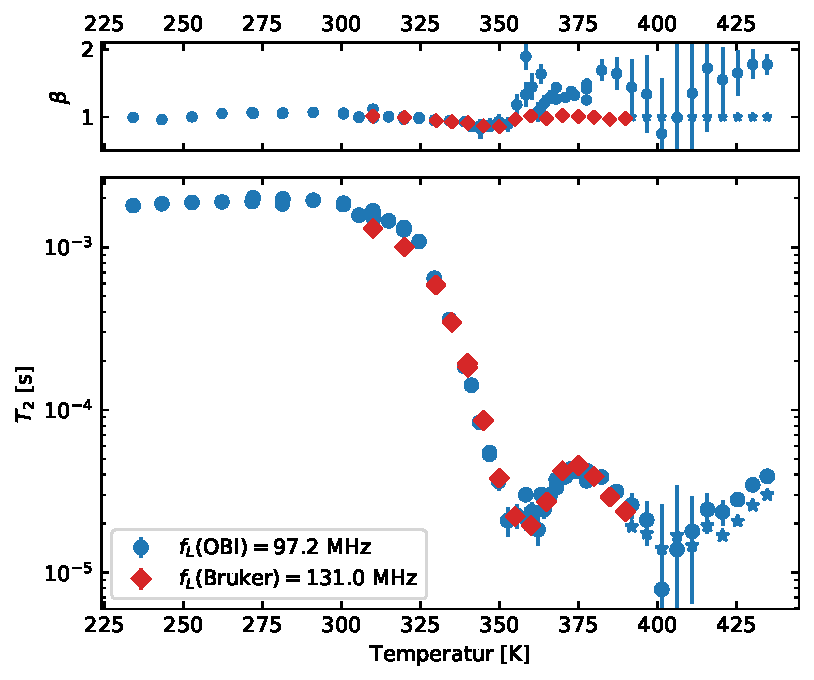
\includegraphics[width=.9\textwidth]{graphics/plot/t2.pdf}
	\end{center}
	\caption{$T_2$ und $\beta$ aus Fits nach Gleichung \eqref{eqn:theo:T_2_fit}. Blaue und rote Symbole zeigen die am OBI- bzw. Bruker-Spektrometer aufgenommen Daten. Bei Temperaturen über $\SI{390}{\kelvin}$ wurden zusätzlich Fits mit einem konstanten $\beta = \SI{1}{}$ erstellt -- diese Werte wurden mit Sternen anstatt Punkten symbolisiert.} \label{fig:res:T_2}
\end{figure}



\section{Untersuchung zur Dynamik von CRN} \label{section:res:F_2}

Mit der Absicht, einen möglichen Betaprozess zu identifizieren, wurden $F_2$-Messungen (siehe Kapitel \ref{section:theo:pulsfolgen}) und pulslängenabhängige Spektren aufgenommen; die verwendeten Methoden und Ergebnisse sollen im Folgenden vorgestellt werden

\subsection{Stimulierte Echos} \label{section:res:stimechos}

Es wurden am OBI-Spektrometer bei $\omega_{L, \text{OBI}} = 2\pi \cdot \SI{97.1722}{MHz}$ $F_2$-Messungen, also stimulierte Echos, über eine Reihe von Temperaturen von $\SI{230}{\kelvin}$ bis $\SI{310}{\kelvin}$ und Evolutionszeiten von $t_p = \SI{50}{\micro s}$ bis $t_p = \SI{1000}{\micro s}$ durchgeführt. Es wurde eine Drei-Puls-Folge verwendet und so sowohl Cos-Cos- als auch Sin-Sin-Korrelationen gemessen.

Bei Evolutionszeiten unter $t_p = \SI{1000}{\micro s}$ und Temperaturen unter $\SI{300}{\kelvin}$ waren die aufgenommenen Daten schwerlich oder gar nicht von $T_1$-Kurven zu unterscheiden, die bei gleicher Temperatur aufgenommen wurden. Es ist möglich, dass mit deutlich mehr Auswertungsaufwand auch hier Ergebnisse erzielt werden könnten; die vorliegende Auswertung soll sich jedoch mit den Temperaturen $\SI{300}{\kelvin}$ und $\SI{310}{\kelvin}$ mit $t_p = \SI{1000}{\micro s}$ befassen. Es wurde je eine Sin-Sin- und Cos-Cos-Messung bei $\SI{300}{\kelvin}$ und $\SI{310}{\kelvin}$ durchgeführt; diese Messreihe wurde als MR1 bezeichnet. Je eine weitere Sin-Sin- und Cos-Cos-Messung wurde bei $\SI{310}{\kelvin}$ aufgenommen. Diese als MR2 bezeichnete Messreihe unterscheidet sich von der ersten in der dreifachen Anzahl der Akkumulationen.

Einen Fit der Form \eqref{eqn:theo:F_2_fit} direkt an die Messwerte anzulegen erwies sich auch bei den höheren Temperaturen als schwierig, daher wurden mehrere Schritte für eine Auswertung durchgeführt. Formel \eqref{eqn:theo:F_2_fit} besteht aus einer Kombination von zwei Kohlrausch-Funktionen, von der jedoch bei der $F_2$-Messung insbesondere die Parameter $\tau_2$ und $\beta_{F_2}$ von Interesse sind. Um einen Fit zur Bestimmung dieser Werte möglich zu machen, soll die Daten von dem Einfluss der $T_1$-Relaxation, welche während auch während der Mischzeit auftritt, bereinigt werden. Dazu wird an die Daten zunächst folgende Funktion gefittet:
\begin{align}
	M_{F_2} (t_m) = M_0 \left[ \exp{ \left(- { \left( \frac{t_m}{\tau_2} \right) }^{\beta_{F_2}} \right)} \right] + M_\text{off} \label{eqn:res:F_2_fit}
\end{align}
Dieser Fit stellt die blaue Kurve in der oberen Hälfte von Abbildung \ref{fig:res:F_2_fit} dar. Die gezeigten Daten entstammen der Messreihe MR2 und wurden am OBI-Spektrometer mit $\omega_{L, \text{OBI}} = 2\pi \cdot \SI{97.1722}{MHz}$ bei einer Temperatur von $\SI{310}{\kelvin}$ und einer Evolutionszeit von $t_p = \SI{1000}{\micro s}$ mit einer Pulsfolge zur Bestimmung der Cos-Cos-Korrelation aufgenommen.
\begin{figure}
	\centering
	\begin{subfigure}{\textwidth}
		\centering
		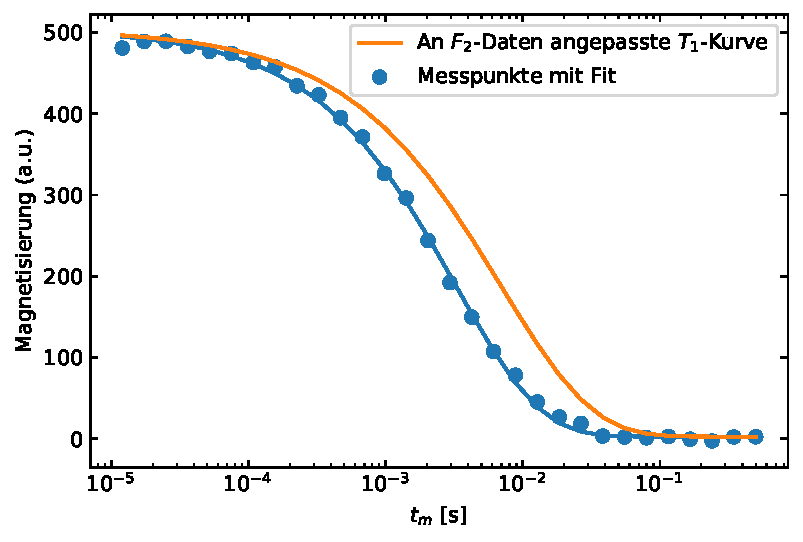
\includegraphics[width=0.8\textwidth]{graphics/plot/f2_310.pdf}
		% \label{fig:res:F_2_tieftemp}
	\end{subfigure} \\
	\begin{subfigure}{\textwidth}
		\centering
		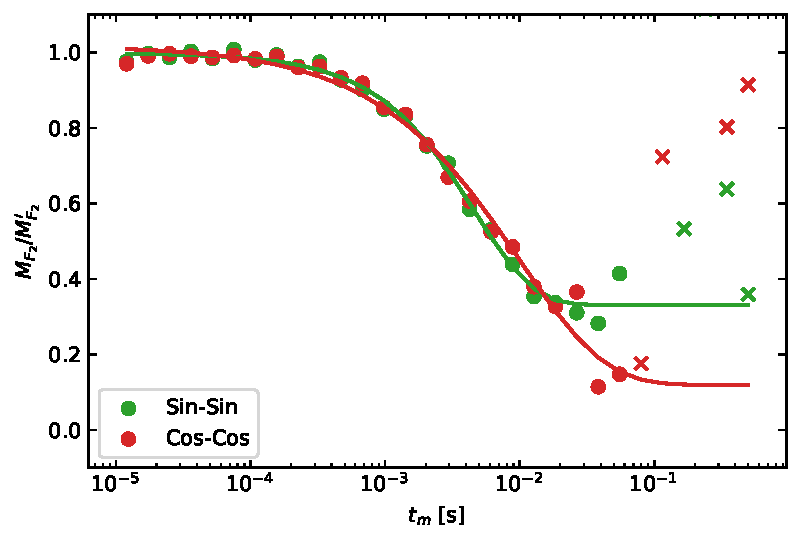
\includegraphics[width=0.8\textwidth]{graphics/plot/f2_fit3.pdf}
		% \label{fig:res:F_2_fit}
	\end{subfigure}
	\caption{Oben: $F_2$-Cos-Cos-Messungen mit $t_p = \SI{1000}{\micro s}$ am OBI-Spektrometer bei $\SI{310}{\kelvin}$ aus der Messreihe MR2. Die blaue Linie zeigt einen Fit an die Daten nach Gleichung \eqref{eqn:res:F_2_fit}, die orangene Linie die angepasste Funktion \eqref{eqn:res:F_2_angp}. Unten: Die Daten nach Gleichungen \eqref{eqn:res:F_2_fit} und \eqref{eqn:res:F_2_angp} durcheinander geteilt. An die entstandenden Daten wurden Kohlrausch-Fits (dargestellt als Linien) angelegt, um Zeitkonstanten zu gewinnen. Stark streuende Werte bei $t_m > \SI{60}{ms}$ wurden nicht in die Fits mit einbezogen und sind als Kreuze dargestellt. Die roten Daten korrespondieren zu den Daten der oberen Grafik; die grünen Daten sind unter den gleichen Umständen aufgenommene Sin-Sin-Messungen.}
	\label{fig:res:F_2_fit}
	\label{fig:res:F_2_T_1}
\end{figure}

Die Werte $\tau_2$ und $\beta_{F_2}$ wurden dann durch $T_1$ und $\beta_{T_1}$ einer $T_1$-Messung gleicher Temperatur ersetzt:
\begin{align}
	M_{F_2}' (t_m) = M_0 \left[ \exp{ \left(- { \left( \frac{t_m}{T_1} \right) }^{\beta_{T_1}} \right)} \right] + M_\text{off} \label{eqn:res:F_2_angp}
\end{align}
Das Resultat ist als orangene Kurve in der gleichen Abbildung gezeigt. Dieses Vorgehen macht es möglich, die $T_1$-Kurve an die $F_2$-Daten anzupassen. Die orangene Kurve symbolisiert, welchen Einfluss $T_1$ allein hat -- von Interesse sind alle weiteren Einflüsse, die zu einem Abfall der Magnetisierung führen. Daher wurden nun die Daten durch die angepasste $T_1$-Kurve geteilt, um den entsprechenden $T_1$-Anteil zu eliminieren. Das Resultat ist in Abbildung \ref{fig:res:F_2_T_1} unten gezeigt; dargestellt sind die Ergebnisse für die Cos-Cos-Messung (welcher die Daten der Grafik in der oberen Hälfte entstammen) und die Sin-Sin-Messung der Messreihe MR2.

An die so gewonnenen Daten kann wiederum ein Kohlrausch-Fit angelegt werden, um über den beschriebenen Umweg zu einer Funktion ähnlich der aus Formel \eqref{eqn:theo:F_2_fit} zu gelangen. Da die Quotienten bei Mischzeiten von über $\SI{60}{\milli s}$ stark streuen -- hier liegen beide Werte nahe 0 -- wurden sie aus dem Fit ausgeschlossen, um das Ergebnis nicht zu beeinträchtigen. Dies wurde in der Abbildung \ref{fig:res:F_2_T_1} durch die Verwendung von Kreuzen anstatt von Punkten symbolisiert.

Die gewonnenen Zeitkonstanten und $\beta$ der Kohlrausch-Fits an die Quotienten finden sich für beide Messreihen in Tabelle \ref{tab:res:F_2} und später in Abbildung \ref{fig:res:dynvgl}.
\begin{table}
	\centering
	\begin{tabular}{lllll}
		\hline
		Temperatur & Sin-Sin $\tau$ & Sin-Sin $\beta$ & Cos-Cos $\tau$ & Cos-Cos $\beta$ \\ \hline
		$\SI{300}{\kelvin}$ (MR1) & $\SI{5.26 (94)}{\milli s}$ & $\SI{0.95 (18)}{}$ & $\SI{3.68 (63)}{\milli s}$ & $\SI{1.30 (34)}{}$ \\
		$\SI{310}{\kelvin}$ (MR1) & $\SI{3.27 (122)}{\milli s}$ & $\SI{1.12 (56)}{}$ & $\SI{9.95 (432)}{\milli s}$ & $\SI{0.74 (21)}{}$ \\
		$\SI{310}{\kelvin}$ (MR2) & $\SI{4.23 (37)}{\milli s}$ & $\SI{1.01 (10)}{}$ & $\SI{3.28 (7)}{\milli s}$ & $\SI{0.71 (1)}{}$ \\
		 \hline
	\end{tabular}
	\caption{Resultate der $F_2$-Messungen. Sin-Sin und Cos-Cos beziehen sich auf die jeweils verwendete Pulsfolge, $\tau$ und $\beta$ sind die mit den Fits bestimmten Parameter der Zeitkonstante und der Streckung der Exponentialfunktion. \label{tab:res:F_2}}
\end{table}

Es ist zu erkennen, dass die Größen zwischen den zwei Messreihen teils mehr schwanken als zwischen zwei Temperaturen oder im Vergleich zwischen Sin-Sin- und Cos-Cos-Pulsfolgen. Da die Unsicherheiten zudem in Fällen beinahe $\SI{50}{\percent}$ erreichen, müssen diese Ergebnisse mit Vorsicht betrachtet werden. Die Werte der Messreihe MR2 sind, wohl aufgrund her höheren Anzahl von Akkumulationen, mit geringeren Unsicherheiten behaftet.



\subsection{Pulslängenabhängige Spektren} \label{section:res:spekdyn}

Eine weitere Untersuchung zu möglicher Dynamik wurde an der sich ändernden Linienform von pulslängenabhängigen Spektren durchgeführt. Während hier nur auf die Bestimmung von Zeitkonstanten eingegangen werden soll, werden die Details von der Linienform von CRN-Spektren im späteren Abschnitt \ref{section:res:spektren} diskutiert.

Es wurde beobachtet, dass Spektren, die mit einem Hahn-Echo mit unterschiedlicher Evolutionszeit $t_p$ aufgenommen wurden, eine unterschiedliche Linienform zeigen. Die Halbwertsbreiten der normierten Spektren sind also evolutionszeitabhängig, und das bei verschiedenen Temperaturen in verschiedenen Maßen. Dies lässt sich in Abbildung \ref{fig:res:spekdyn_305K} erkennen, wo normierte, pulslängenabhängige Spektren für die Temperaturen $\SI{305}{\kelvin}$ oben bzw. $\SI{325}{\kelvin}$ unten gezeigt sind. Die Daten wurden am OBI-Spektrometer mit $\omega_{L, \text{OBI}} = 2\pi \cdot \SI{97.1722}{MHz}$ aufgenommen und mit Gaußfunktion mit einer Breite von $\SI{500}{Hz}$ apodisiert. Diese Faltung sorgt für eine Verbreiterung der Spektren, welche zwar die Auflösung, aber auch das Rauschen verringert.
\begin{figure}
	\centering
	\begin{subfigure}{\textwidth}
		\centering
		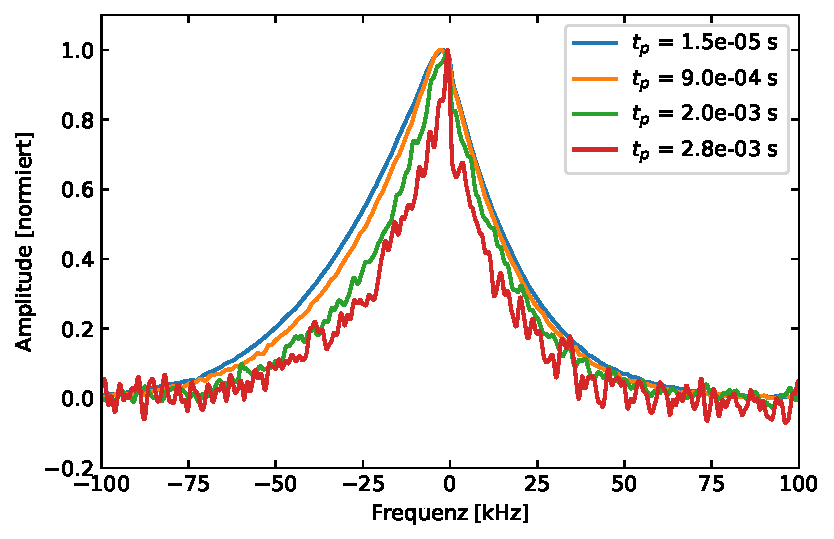
\includegraphics[width=.9\textwidth]{graphics/plot/spekdyn_305K2.pdf}
	\end{subfigure} \\
	\begin{subfigure}{\textwidth}
		\centering
		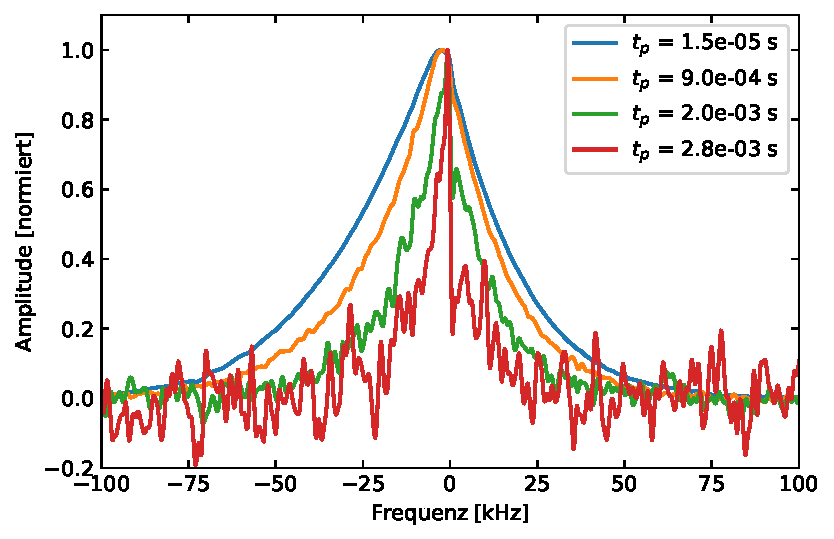
\includegraphics[width=.9\textwidth]{graphics/plot/spekdyn_325K2.pdf}
	\end{subfigure}
	\caption{Änderung der Linienform der mit einem Hahn-Echo aufgenommenen Spektren bei $\SI{305}{\kelvin}$ (oben) und bei $\SI{325}{\kelvin}$ (unten) in Abhängigkeit der Evolutionszeit $t_p$. Die Daten wurden am OBI-Spektrometer mit $\omega_{L, \text{OBI}} = 2\pi \cdot \SI{97.1722}{MHz}$ aufgenommen und auf ihr Maximum normiert.}
	\label{fig:res:spekdyn_305K}
	\label{fig:res:spekdyn_325K}
\end{figure}

Zur Untersuchung der Evo\-lu\-tions\-zeit-Ab\-häng\-ig\-keit wurde für jede Temperatur die Halbwertsbreite -- als Maß für die Linienform -- gegen die Evolutionszeit $t_p$ aufgetragen. An diese Daten wurden Kohlrausch-Fits angelegt, die als durchgezogene Linien, zusammen mit dem Daten, in Abbildung \ref{fig:res:spekdyn_fits} zu sehen sind. Alle Spektren wurden am OBI-Spektrometer aufgenommen. Da die Spektren bei zunehmenden Pulslängen ein immer schlechteres Sig\-nal-Rausch-Ver\-hält\-nis aufweisen -- beispielhaft zu erkennen in der unteren Hälfte der Abbildung \ref{fig:res:spekdyn_325K} für $t_p = \SI{2.7}{\milli s}$ --, wurden die verwendeten Evolutionszeiten auf $\SI{2}{\milli s}$ begrenzt. 
\begin{figure}
	\begin{center}
		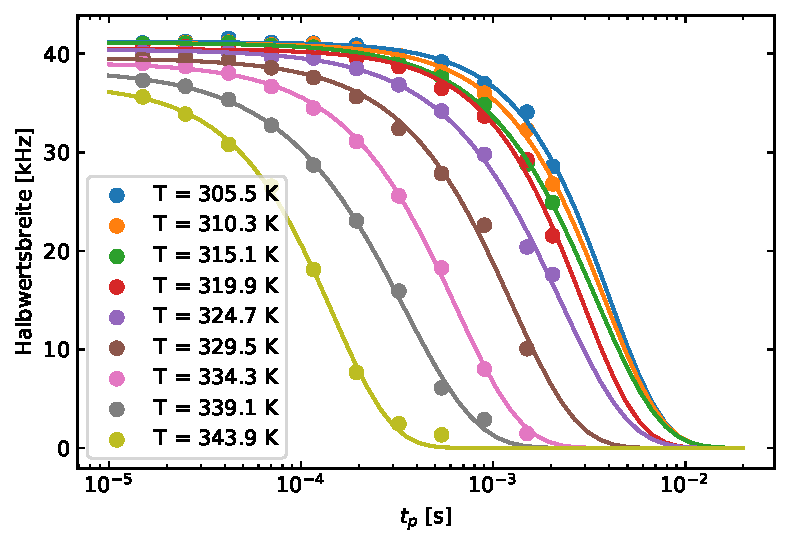
\includegraphics[width=.9\textwidth]{graphics/plot/spekdyn_fits2.pdf}
	\end{center}
	\caption{Halbwertsbreiten der Spektren in Abhängigkeit von $t_p$. An diese Daten wurden Kohlrausch-Fits angelegt, dargestellt als durchgezogene Linien.} \label{fig:res:spekdyn_fits}
\end{figure}

Es wurde eine weitere, ähnliche Auswertung durchgeführt, wobei anstatt der Halbwertsbreite die Amplitude bei einer bestimmten Frequenz (beispielsweise bei $\SI{-15}{\kilo Hz}$) als Variable genommen wurde. Die Ergebnisse glichen der der Halbwertsbreiten-Betrachtung, waren aber durchgehend mit Unsicherheiten in Größenordnung der eigentlichen Werte behaftet. Dies lässt sich durch die stark verrauschten Spektren bei hohen Evolutionszeiten erklären, die zu stark schwankenden Amplituden führen, welche wiederum einen guten Fit der Daten schwierig gestalten. Es ist die Untersuchung der Halbwertsbreiten dieser Methode vorzuziehen.



\subsection{Auswertung der experimentell bestimmten Zeitkonstanten} \label{section:res:dynausw}

Werden die bestimmten Zeitkonstanten der $T_1$-, $T_2$-, $F_2$- und $t_p$-abhängigen Spek\-trums-Mess\-un\-gen zusammen aufgetragen, ergibt sich das in Abbildung \ref{fig:res:dynvgl} gezeigt Bild.
\begin{figure}
	\begin{center}
		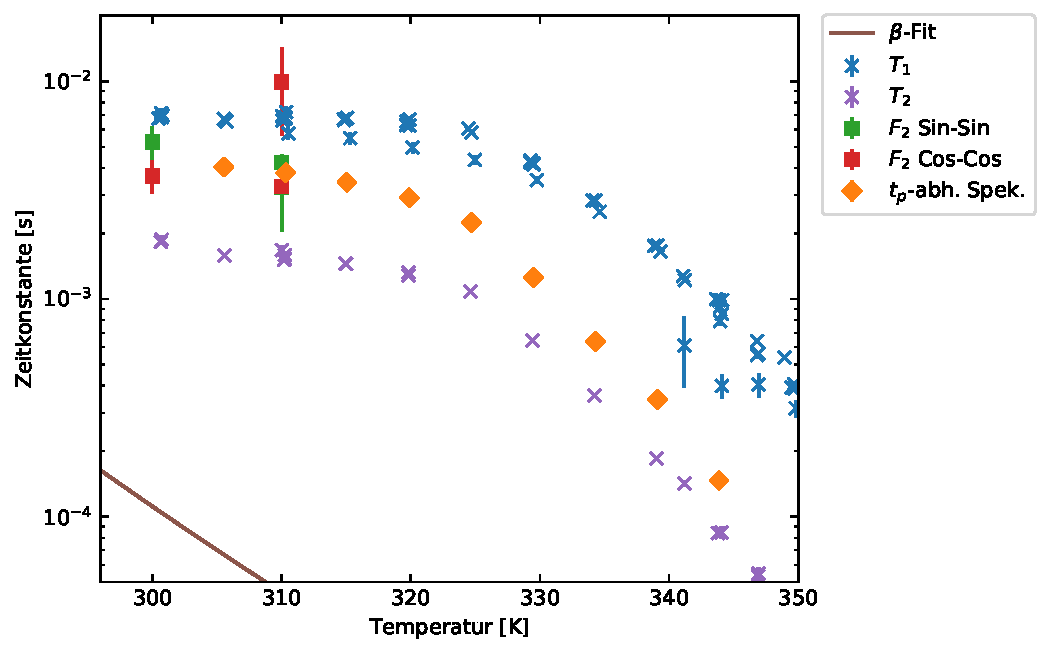
\includegraphics[width=.9\textwidth]{graphics/plot/dyn.pdf}
	\end{center}
	\caption{Vergleich der gewonnenen Zeitkonstanten.
	
	Die braune Linie entspricht der gestrichelten Linie aus Abbildung \ref{fig:einl:zuernpaper}, welche ein Fit an Zeitkonstanten eines Betaprozesses ist.} \label{fig:res:dynvgl}
\end{figure}
Alle bestimmten Zeitkonstanten liegen -- im Rahmen der Unsicherheiten -- zwischen den bestimmten $T_1$- und $T_2$-Werten. Diese Unsicherheiten sind bei fast allen Messungen, mit Ausnahme der $F_2$-Messungen, unter der verwendeten Symbolgröße und können vernachlässigt werden. Gründe für die höheren Unsicherheiten der $F_2$-Messungen könnten die mehrschrittige Auswertung und die verrauschten Signale bei hohen Evolutionszeiten sein.

Ab $\SI{320}{\kelvin}$ bis $\SI{330}{\kelvin}$ zeigen alle Zeitkonstanten einen Übergang zu kürzeren Zeiten, der wohl mit der höheren Bewegung der Atome in der Nähe der Glasübergangstemperatur von $T_g = \SI{333}{\kelvin}$ einhergeht. Dieser Effekt ist auch als Bewegungsverschmälerung in Spektren zu sehen (vgl. Abbildung \ref{fig:res:spek_fwhm}).

Die braune Linie stellt dabei einen Fit durch die in Abbildung \ref{fig:einl:zuernpaper} gezeigten, zum Betaprozess gehörenden Werte dar. Die Linie kann eine Abschätzung zu geben, in welcher Größenordnung der Prozess im untersuchten Temperaturbereich liegt, sollte sich der angedeutete Trend im Arrhenius-Diagramm \ref{fig:einl:zuernpaper} linear fortsetzen. Wie zu erkennen, befindet sich keine der bestimmten Zeitkonstanten in der entsprechenden Größenordnung. Dies bedeutet möglicherweise, dass der Prozess mit den hier verwendeten Methoden nicht detektiert werden kann -- ein zu geringer Einfluss könnte der Grund sein. Weitere Untersuchungen sind nötig, um diese Frage abschließend klären zu können.



\section{Linienform von experimentellen und simulierten CRN-Spektren} \label{section:res:spektren}

Das zweite Ziel dieser Arbeit ist die Untersuchung der Linienform von CRN-Spek\-tren. Bei der Auswertung von Spektren wurde eine zunächst ungewöhnlich erscheinende Verbreiterung derselben in einem Temperaturbereich beobachtet, wo, aufgrund von Bewegungsverschmälerung, eher kleinere Halbwertsbreiten zu erwarten wären. Zur Untersuchung der Gegebenheiten wurden, neben einer Vielzahl von experimenteller Spektren, Computer-Simulationen angefertigt und versucht, eine theoretische Erklärung der Daten zu bieten.

\begin{figure}
	\begin{center}
		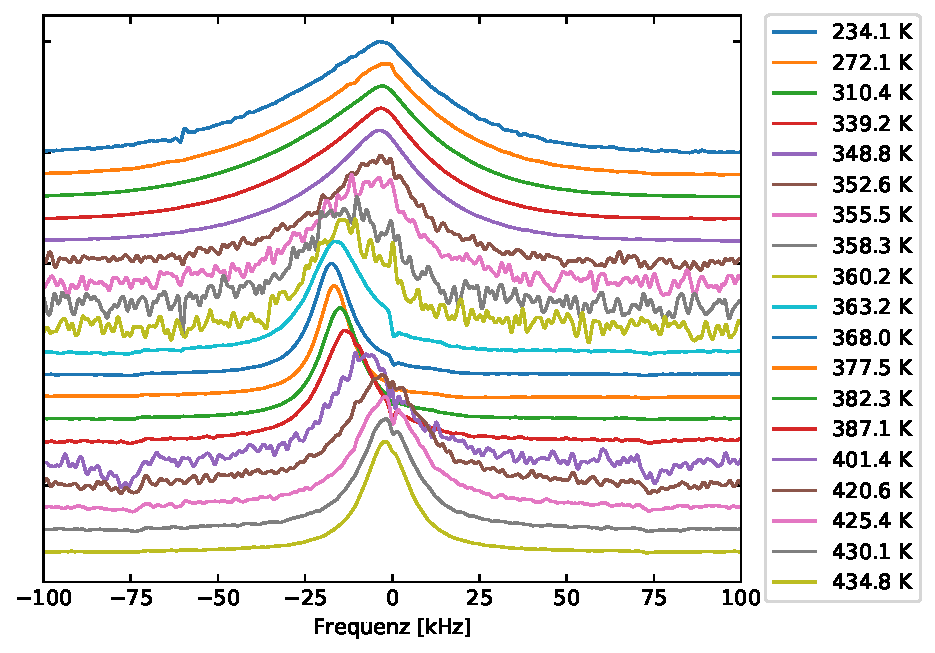
\includegraphics[width=\textwidth]{graphics/plot/spek_lineshape.pdf}
	\end{center}
	\caption{Vergleich der Linienform von am OBI-Spektrometer aufgenommen Spektren.} \label{fig:res:spek_linienform}
\end{figure}
Um eine Übersicht zu schaffen, werden zuerst die Linienformen der Spektren aus den verschiedenen Quellen in Abhängigkeit der Temperatur präsentiert. Abbildung \ref{fig:res:spek_linienform} zeigt die am OBI-Spektrometer aufgenommenen Spektren; die Temperaturen reichen von etwa $\SI{234}{\kelvin}$ bis etwa $\SI{435}{\kelvin}$. Sie wurden mit einem Hahn-Echo mit einer Evolutionszeit von $t_p = \SI{15}{\micro s}$ aufgenommen und mit $\SI{500}{Hz}$ apodisiert. Es wurden je $\SI{8192}{}$ Datenpunkte mit einer Frequenz von $\SI{2}{MHz}$ erstellt. Die Spektren wurden in mehreren Messreihen aufgenommen und stellen eine repräsentative Auswahl dar, die es erlaubt, den Verlauf der Linienform nachzuvollziehen, ohne zu stark an Übersicht zu verlieren.

Bei tiefen Temperaturen ist eine Form zu beobachten, die der des Czjzek-Spektrums aus Kapitel (***) ähnelt. Diese hält sich über weite Temperaturen, von etwa $\SI{235}{\kelvin}$ bis etwa $\SI{350}{\kelvin}$, fast unverändert. Bei steigenden Temperaturen ändert sich die Linienform, sie nimmt die einer Lorentz-Funktion
\begin{align}
	L(f) = \frac{1}{\pi \gamma} \cdot \frac{\gamma^2}{\gamma^2 + (f - f_0)^2} \label{eqn:res:lorentz}
\end{align}
an, während die Spektren gleichzeitig schmaler werden und sich der Schwerpunkt zu niedrigeren Frequenzen verschiebt. Diese Bewegung findet ein Ende bei etwa $\SI{367}{\kelvin}$: Zu höheren Temperaturen verbreitern sich die Spektren wieder, ehe sie ab $\SI{410}{\kelvin}$ wieder schmaler werden. Der Schwerpunkt verschiebt sich ab 375K wieder gegen $\SI{0}{Hz}$, wo er ab 400K verweilt. Die Linienform ändert sich nicht mehr.

Es ist auffällig, dass die Qualität der Spektren stark mit der Temperatur schwankt. Zwischen $\SI{235}{\kelvin}$ und $\SI{350}{\kelvin}$, $\SI{363}{\kelvin}$ und $\SI{387}{\kelvin}$, sowie zwischen $\SI{430}{\kelvin}$ und $\SI{435}{\kelvin}$ weisen die Spektren vergleichsweise geringes Rauschen und somit eine glattere Form auf. Die abschnittweise höheren Schwankungen lassen sich durch $T_2$-Minima (siehe Abbildung \ref{fig:res:T_2}) bei den entsprechenden Temperaturen erklären -- diese sorgen für einen schnellen Abfall des Signals und entsprechend verrauschte Spektren.

\begin{figure}
	\begin{center}
		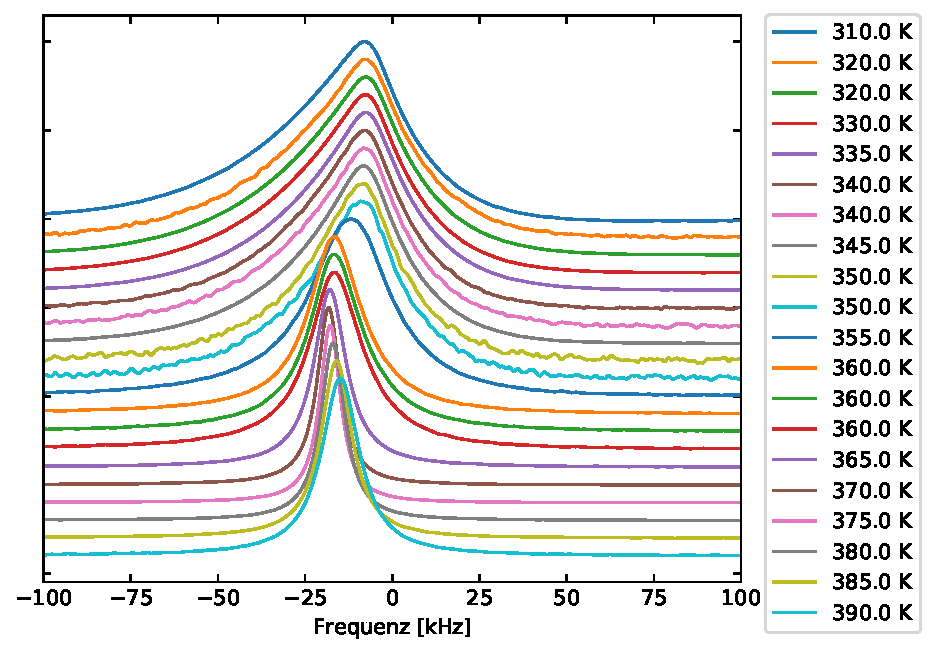
\includegraphics[width=\textwidth]{graphics/plot/bruker_lineshape.pdf}
	\end{center}
	\caption{Vergleich der Linienform von am Bruker-Spektrometer aufgenommen Spektren.} \label{fig:res:bruker_linienform}
\end{figure}
Die am Bruker-Spektrometer aufgenommenen Spektren decken einen Temperaturbereich von $\SI{310}{\kelvin}$ bis $\SI{390}{\kelvin}$ ab und wurden ebenfalls mit einem Hahn-Echo mit einer Evolutionszeit von $\SI{15}{\micro s}$ erstellt und mit $\SI{500}{Hz}$ apodisiert. Hier wurden je $\SI{4096}{}$ Datenpunkte mit einer Frequenz von $\SI{0.5}{MHz}$ aufgenommen. Da mit diesem Spektrometer weitaus weniger Spektren erstellt wurden als mit dem OBI-Spektrometer, können in Abbildung \ref{fig:res:bruker_linienform} alle erstellten Spektren präsentiert werden.

Der Verlauf der Linienform gleicht der beschriebenen in dem entsprechenden Temperaturbereich gut. Es ist das geringe Rauschen der Spektren zu beachten, das, wie auch insbesondere die $T_2$-Daten, ein Beleg für hohe Datenqualität des Bruker-Spektrometers in diesem Kontext ist.

Als Ergänzung zu den experimentellen Daten wurden Spektren simuliert. Dazu wurde die in Kapitel (***) vorgestellte Simulations-Software verwendet. Es wurden FIDs mit $\SI{4096}{}$ Datenpunkten mit einem Abstand von je $\SI{0.5}{\micro s}$, was einer Frequenz von $\SI{2}{MHz}$ entspricht, aufgenommen. Um einen Mittelwert zu bilden, wurden, je nach Spektrum, zwischen $10^{7}$ und $10^{9}$ einzelne Trajektorien gemittelt. Als Modell wurde ein isotroper Zufallssprung gewählt, welcher eine Czjzek-Verteilung als Ausgangspunkt hat; dieses war der simulierten Quadrupol-Wechselwirkung zweiter Ordnung ausgesetzt. Zur Bestimmung der Lebensdauer eines bestimmten Zustandes wurde eine Exponentialverteilung genutzt, deren Parameter, die Lebenszeit, eine Verknüpfung mit Temperaturen ermöglicht. Es wurde eine Vogel-Fulcher-Funktion für die Lebenszeit mit den Parametern für CRN aus \cite{PIMENOV199793} verwendet. Zur besseren Vergleichbarkeit werden im Folgenden die Spektren mit den so berechneten Temperaturen anstatt mit den Lebenszeiten referenziert. Die resultierenden Spektren sind in Abbildung \ref{fig:res:sim_linienform} zu sehen. Da die Breite der Spektren in der Simulation mit nur einem frei wählbaren Parameter bestimmt wird, wurde sie durch das Vergleichen der Form bei tiefen Temperaturen normiert.
\begin{figure}
	\begin{center}
		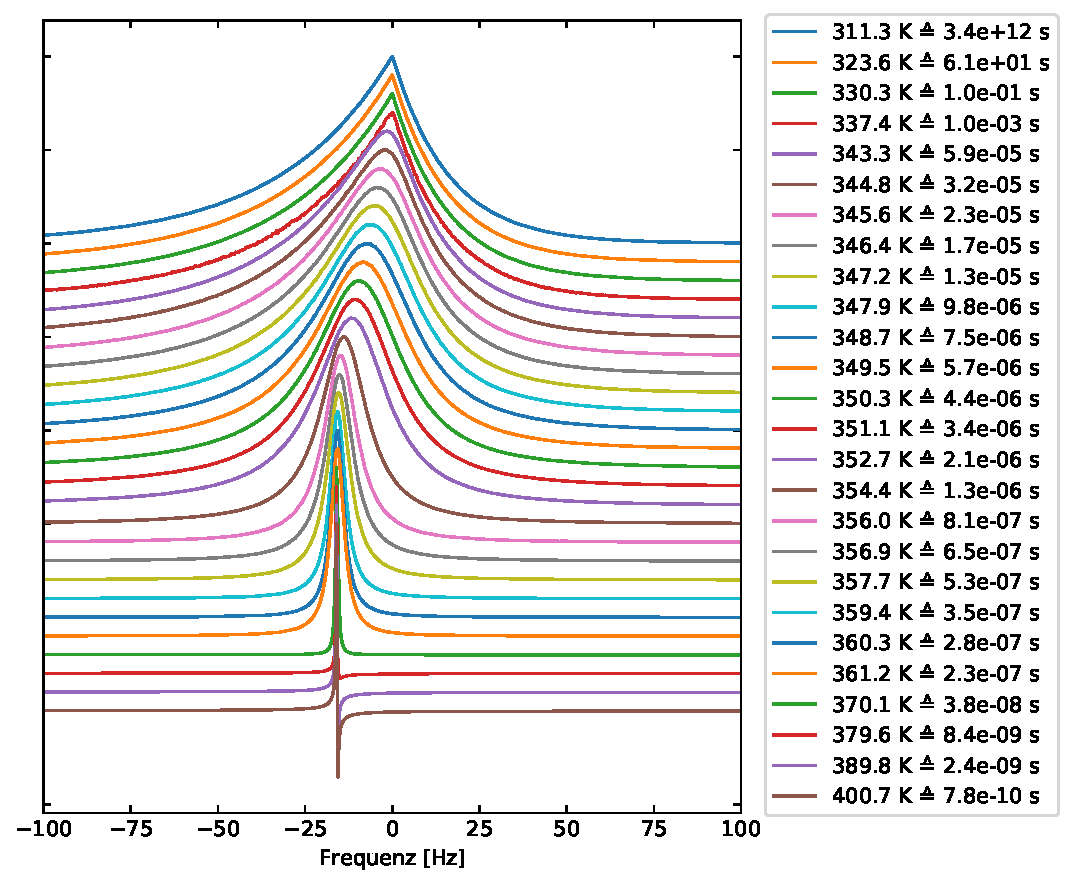
\includegraphics[width=\textwidth]{graphics/plot/sim_lineshape.pdf}
	\end{center}
	\caption{Vergleich der Linienform von mit Simulationen erstellte Spektren. Die angegebenen Temperaturen wurden mithilfe von den in Kapitel \ref{section:res:theorie} beschriebenen $\tau_c$ aus den verwendeten $\tau$ bestimmt.} \label{fig:res:sim_linienform}
\end{figure}

Bei tiefen Temperaturen gleichen die simulierten Spektren den experimentellen; dies wurde schon in \cite{joachim_master} gefunden. Auch ist der Übergang zur Lorentz-Form, verbunden mit der Verschiebung des Schwerpunkts und Verschmälerung der Spektren bei etwa der gleichen Temperatur von $\SI{350}{\kelvin}$ zu beobachten. Im Gegensatz zu den experimentellen Spektren werden die simulierten Spektren mit steigender Temperatur jedoch immer schmaler und ändern den Schwerpunkt nicht mehr.


Um eine quantitative Behandlung der Spektren zu ermöglichen, wurden zwei Messgrößen verwendet: Die Halbwertsbreite (also die Breite auf der Höhe der Hälfte des Maximums) und der Schwerpunkt der Spektren. Um bei den stark verrauschten Spektren des OBI-Spektrometers zwischen $\SI{350}{\kelvin}$ und $\SI{360}{\kelvin}$ und zwischen $\SI{390}{\kelvin}$ und $\SI{430}{\kelvin}$ gut vergleichbare Werte zu erhalten, wurde ein Lorentz-Fit nach Gleichung \eqref{eqn:res:lorentz} mit einer least-squares-Methode an die Spektren angelegt. So entspricht $2 \gamma$ der Halbwertsbreite und das Maximum $f_0$, aufgrund der Symmetrie der Funktion, dem Schwerpunkt. Die so gewonnenen Halbwertsbreiten sind in Abbildung \ref{fig:res:spek_fwhm} zu sehen.
\begin{figure}
	\begin{center}
		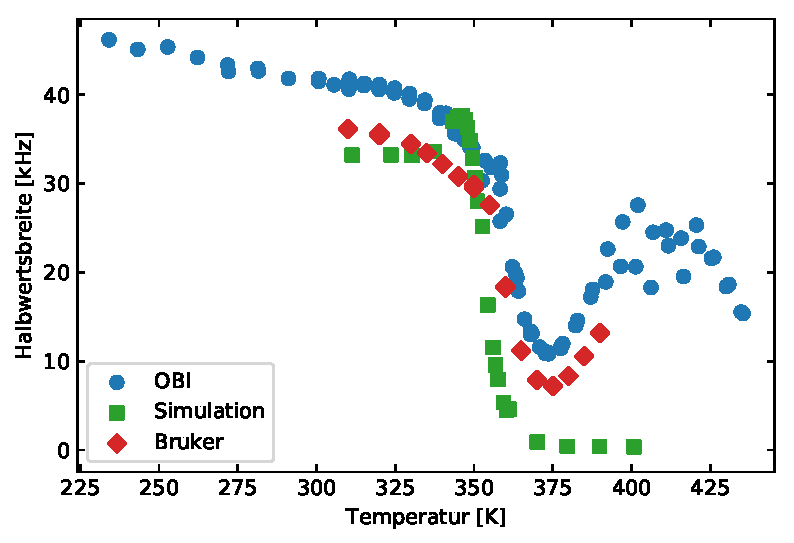
\includegraphics[width=.9\textwidth]{graphics/plot/fwhm.pdf}
	\end{center}
	\caption{Die Halbwertsbreite der Spektren. Blaue und rote Symbole kennzeichnen am OBI- bzw. Bruker-Spektrometer aufgenommene Spektren, grüne Symbole stammen von simulierten Spektren. Der auffälligste Unterschied zwischen experimentellen und simulierten Spektren ist das zusätzliche Maximum bei hohen Temperaturen bzw. dessen Fehlen.} \label{fig:res:spek_fwhm}
\end{figure}

Es ist zu erkennen, dass die Werte der Halbwertsbreite etwa dem entsprechen, was nach einer Betrachtung der Spektren zu erwarten wäre: Von einem Spektrum mit etwa $\SI{40}{kHz}$ Breite bei niedrigen Temperaturen gehen die Werte zu einem Minimum von etwa $\SI{10}{kHz}$ bei etwa $\SI{375}{\kelvin}$ über, um nach einem lokalen Maximum von rund $\SI{20}{kHz}$ bei etwa $\SI{400}{\kelvin}$ erneut abzufallen.

Diesem Verlauf der am OBI-Spektrometer aufgenommenen Spektren folgen auch die Halbwertsbreiten der am Bruker-Spektrometer produzierten Daten. Letztere liegen allerdings konstant bei niedrigeren Werten. Das Verhältnis entspricht aber auch nicht durchgehend dem Verhältnis $4:3$, was die entsprechend unterschiedlichen Larmorfrequenzen suggerieren würden; es liegt bei tiefen Temperaturen etwas niedriger und bei höheren Temperaturen etwas höher. So ist im Bereich zwischen $\SI{310}{\kelvin}$ und $\SI{350}{\kelvin}$ ein Verhältnis von etwa $\SI{1.15}{}:1$ zu finden, zwischen $\SI{360}{\kelvin}$ und $\SI{390}{\kelvin}$ ein Verhältnis von $\SI{1.45}{}:1$ bis $\SI{1.55}{}:1$. Messungen an einem $\SI{600}{MHz}$-Spektrometer wären hilfreich, um fundiertere Aussagen über Larmorfrequenz-abhängige Effekte treffen zu können.

Der Verlauf der Halbwertsbreiten der simulierten Spektren unterscheidet sich deutlich von dem der experimentellen Spektren. Während der grobe Verlauf übereinstimmt -- von breiten Spektren bei tiefen Temperaturen zu schmalen Spektren bei höheren Temperaturen -- sind bei genauerer Betrachtung starke Abweichungen zu sehen. Die simulierten Spektren werden zu höheren Temperaturen zunehmend schmaler und näheren sich einem Delta-Peak, während die Breiten der experimentellen Spektren ein weiteres Maximum aufweisen. Zudem ist ein Maximum der Halbwertsbreite der simulierten Spektren bei etwa $\SI{345}{\kelvin}$ zu beobachten, während die Halbwertsbreite der experimentellen Spektren einen fließenden Übergang der Breite von hohen zu tiefen Temperaturen zeigen.

Es sollte darauf aufmerksam gemacht werden, dass die Halbwertsbreite stark von der Form der Spitze beeinflusst wird, welche das Maximum und damit die Hälfte des Maximums bestimmt. Sind, wie bei den simulierten Spektren, extrem gut definierte Maxima zu sehen, drückt dies den Wert der Halbwertsbreiten im Vergleich zu den experimentellen Halbwertsbreiten nach unten. Dies erklärt den Abfall der Halbwertsbreiten der simulierten Spektren zu tieferen Temperaturen: Hier sind die scharfen Spitzen der Czjzek-Spektren gut ausgeprägt, sodass die Halbwertsbreite der Spektren beim Übergang zur abgerundeten Lorentz-Form ein Maximum durchläuft. Die experimentellen Spektren hingegen zeigen aufgrund von experimentellen Beschränkungen wie der Auflösung, und möglicherweise durch weitere Effekte, bei niedrigeren Temperaturen keine perfekte Spitze und daher auch keinen Peak in der Halbwertsbreite beim Übergang zur Lorentz-Form.

\par\bigskip

In Abbildung \ref{fig:res:spek_mean} sind die Schwerpunkte der Spektren aufgetragen. Diese wurden mit Hilfe von numerischer Integration nach der Simpsonregel bestimmt. Bei stark verrauschten Spektren, wo dieses Vorgehen wenig Erfolg verspricht -- es wird eher der Schwerpunkt der Schwankungen bestimmt als der des Signals --, wurden wieder Lorentz-Fits ausgenutzt, deren Parameter $f_0$ der Schwerpunkt ist.
\begin{figure}
	\begin{center}
		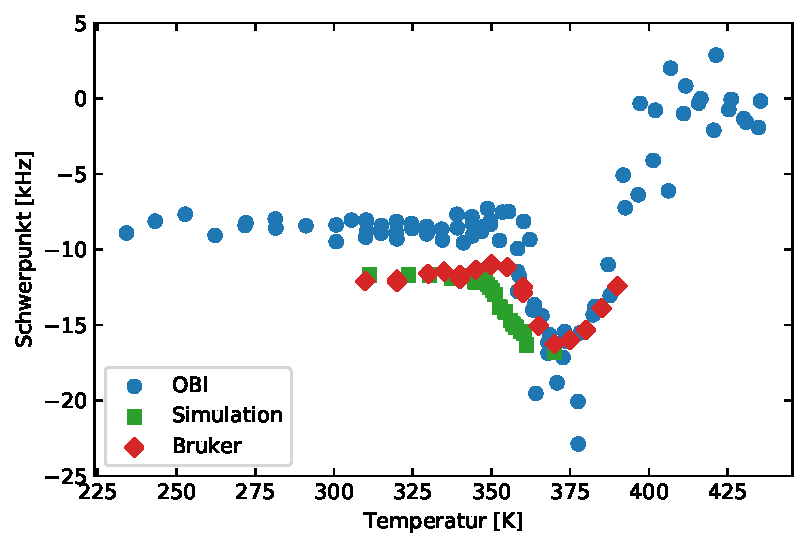
\includegraphics[width=.9\textwidth]{graphics/plot/mean.pdf} 
	\end{center}
	\caption{Die Halbwertsbreite der Spektren. Blaue und rote Symbole kennzeichnen am OBI- bzw. Bruker-Spektrometer aufgenommene Spektren, grüne Symbole stammen von simulierten Spektren. Während der Schwerpunkt der experimentellen Spektren zu hohen Temperaturen gegen $\SI{0}{\kilo Hz}$ geht, verbleibt der Schwerpunkt der simulierten Spektren bei etwa $\SI{-16}{\kilo Hz}$.} \label{fig:res:spek_mean}
\end{figure}

Allen drei Kurvenverläufen ist gleich, dass sie bei tieferen Temperaturen bis etwa $\SI{360}{\kelvin}$ einen konstanten Wert zeigen, ehe sich der Schwerpunkt zu niedrigeren Frequenzen von etwa $\SI{-16}{\kilo Hz}$ verschiebt, was mit dem Übergang von der Czjzek-Form des Spektrums zur Lorentz-Form einhergeht. Die spezifischen konstanten Werte der tieferen Temperaturen unterscheiden sich jedoch zwischen den Daten des OBI-Spektrometers mit einem Schwerpunkt von etwa $\SI{-8}{\kilo Hz}$ und den Daten des Bruker-Spektrometers und der Simulation mit einem Schwerpunkt von etwa $\SI{-12}{\kilo Hz}$. Auch in diesem Kontext könnten Messungen an Spektrometern mit unterschiedlichen Larmorfrequenzen helfen, um beispielsweise den Einfluss der chemischen Verschiebung auf die Position der Schwerpunkte zu untersuchen.

Ab etwa $\SI{375}{\kelvin}$ ist eine Bewegung des Schwerpunkts der experimentellen Spektren zum Nullpunkt zu erkennen, die die Spektren des OBI-Spektrometers aufgrund des größeren abgedeckten Temperaturbereichs auch erreichen. Die simulierten Spektren verbleiben jedoch bei dem Wert von $\SI{-16}{\kilo Hz}$, der bei $\SI{370}{\kelvin}$ erreicht wird.

Auch hier ist einschränkend zu sagen, dass die Werte der Schwerpunkte aufgrund von externen Faktoren instabil sind, mehr noch als die Halbwertsbreiten. Wie in Kapitel \ref{section:exp:weiterverarbeitung} erwähnt, wird eine Phasenanpassung des Real- und Imaginärteils durchgeführt, um ein maximales Signal zu garantieren und mögliche Schwankungen der Phase durch experimentelle Einflüsse auszugleichen. Allerding kann eine Abweichung von $\pm \SI{1}{\degree}$ vom Optimalwert unter den schlechtesten Umständen eine Verschiebung des Schwerpunkts um $\SI{1}{\kilo Hz}$ bewirken. Diese Empfindlichkeit gegenüber kleinen Änderungen bedeutet, dass Schwankungen der dargestellten Werte nicht auszuschließen sind; die groben Merkmale der Kurvenverläufe können aber leicht durch eine Betrachtung der Spektren bestätigt werden.




\section{Vergleich von CRN-Spektren mit theoretischen Überlegungen} \label{section:res:theorie}

Die experimentellen Ergebnisse sollen mit den theoretischen Überlegungen vergleichen werden. Dazu wurden die in Kapitel \ref{section:theo:qww} beschriebenen Funktionen für $T_1$, Halbwertsbreite und Schwerpunkt verwendet. Um eine Übereinstimmung zur Theorie feststellen zu können, müssen sich alle Datensätze mit dem gleichen Satz geteilter Parameter beschreiben lassen. Im Falle der Spektraldichte $J_\text{BPP}$ ist dies $C_Q$; für $J_\text{CC}$ und $J_\text{CD}$ sind $\alpha$ bzw. $\gamma$ zusätzliche Parameter.

Für den Parameter $\eta$ der Spektraldichten wurde $\eta^2 = 42 - 24 \sqrt{3} \approx \SI{0.43}{}$ \cite{caer} verwendet. Nach \cite{PIMENOV199793} wird für CRN für die Korrelationszeit $\tau_c$ ein Vogel-Fulcher-Gesetz
\begin{align}
	\tau_c = \tau_{co} \exp \left( \frac{D T_\text{VF}}{T-T_\text{VF}} \right)
\end{align}
mit dem strength index $D = \SI{3.5}{}$, der Vogel-Fulcher-Temperatur $T_\text{VF} = \SI{294}{K}$ und dem Frequenzfaktor $\tau_{co} = \SI{5.1e-14}{s}$ angenommen. Diese Werte wurden durch dielektrische Spektroskopie gewonnen.

Am $T_1$-Minimum nach Gleichung \eqref{eqn:bpp} gilt $\omega \tau_c \approx \SI{0.61}{}$ \cite[S. 629]{omegatau061}. Das $T_1$-Minimum kann in den OBI-Daten bei etwa $T_{T_1 \text{min}} = \SI{410}{K}$ gefunden werden; die Larmorfrequenz liegt bei $\omega_L = 2\pi \cdot \SI{97.1722}{MHz}$, was bedeutet, dass bei $T_{T_1 \text{min}}$ gilt $\tau_c \approx \sfrac{\SI{0.61}{}}{\omega_L} \approx \SI{1.0}{\nano s}$. Vergleicht man das Vogel-Fulcher-Gesetz mit diesem Punkt, lässt sich erkennen, dass eine gute Übereinstimmung vorliegt.

\begin{wrapfigure}{r}{0.5\textwidth}
	\vspace{-20pt}
	\begin{center}
		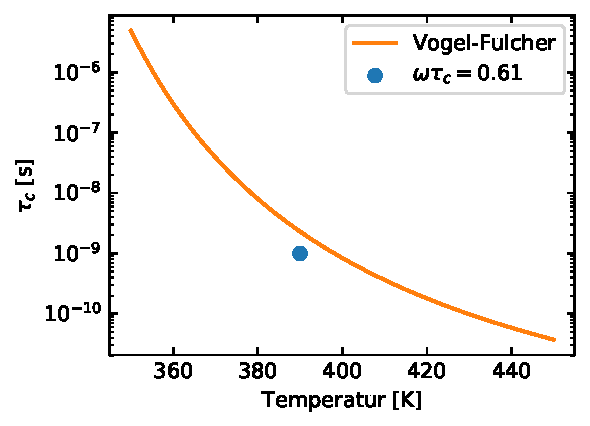
\includegraphics[width=0.49\textwidth]{graphics/plot/vftau.pdf}
	\end{center}
	\vspace{-20pt}
	\caption{Vergleich von Zeitkonstante aus $T_1$-Minimum, und Vogel-Fulcher-Gesetz für CRN mit Parametern nach \cite{PIMENOV199793} in orange und Parametern nach \cite{crn_augsburg} in grün. \label{fig:korrelationszeiten}}
\end{wrapfigure}
Ein Vergleich mit den Parametern $D = \SI{4.72}{}$, $T_\text{VF} = \SI{285}{K}$ und $\tau_{co} = \SI{1.15e-14}{s}$ nach \cite{crn_augsburg}, ebenfalls bestimmt durch dielektrische Spektroskopie, ist in den Abbildungen \ref{fig:korrelationszeiten} und \ref{fig:res:theorie_j} zu sehen. Während leichte Unterschiede zu erkennen sind, ändert sich das Gesamtbild wenig, weswegen sich diese Ausführungen auf den ersten Parametersatz beschränken.




Führt man zunächst einen Vergleich der Halbwertsbreiten mit der Theorie durch, lässt sich leicht feststellen, dass signifikante Unterschiede zu beobachten sind: Die gemessenen Halbwertsbreiten sind ab $\SI{360}{\kelvin}$ aufwärts deutlich größer als vorhergesagt. Dies liegt am Einfluss des kurzen $T_1$ von etwa $\SI{50}{\micro s}$, welches mit der zusätzlich Relaxation zur Verbreiterung des Spektrums beiträgt.

Um einen Vergleich mit der Theorie dennoch durchführen zu können, wurde versucht den Einfluss von $T_1$ rechnerisch zu eliminieren. Im Bereich des Einflusses lassen sich die Spektren gut mit einem Lorentz-Fit (vgl. Gleichung \eqref{eqn:res:lorentz}) nähern. Die Fouriertransformierte hiervon ist eine gedämpfte Schwingung mit der Halbwertsbreite $2 \gamma_0 = a/\pi$:
\begin{align}
	h(t) & = \exp{(-a |t|)} \cos{(2 \pi f_0 t)} \\
	H(t) & = \int_{-\infty}^{\infty} h(t) \exp{i 2 \pi f t} \text{d} t \\
	H(f) & = \frac{2}{a} \cdot \frac{(a/2\pi)^2}{((a/2\pi)^2) + (f - f_0)^2}
\end{align}

Diese gedämpfte Schwingung soll durch eine normierte Kohlrausch-Funktion
\begin{align}
	f(t) = \exp{\left( {\left(-\frac{t}{T_1} \right)}^\beta \right) },
\end{align}
welche für Fits an $T_1$ verwendet werden kann, geteilt werden. Da die Messung der Signale per Definition immer bei 0 beginnt, kann $t$ durch $|t|$ ersetzt werden. Für eine vereinfachte Rechnung wird hier wird $\beta = 1$ angenommen, was in der Regel eine annehmbare Näherung darstellt.
\begin{align}
	h'(t) &= \exp{(-a \lvert t \rvert)} \cdot \cos{(2 \pi f_0 t)} \cdot \exp{\left(\frac{|t|}{T_1} \right)} \\
	&= \exp{\left(- \left(a - \frac{1}{T_1}\right) |t|\right)} \cos{(2 \pi f_0 t)}
\end{align}
Wird der Quotient der Funktionen zurück in den Frequenzraum transformiert, ergibt sich $a' = a - \sfrac{1}{T_1}$ und damit die modifizierte Halbwertsbreite $2\gamma = 2\gamma_0 - \frac{1}{\pi T_1}$.

Dies bedeutet, dass für die Korrektur lediglich die schon vorliegenden Halbwertsbreiten mit $T_1$-Werten der passenden Temperaturen modifiziert werden müssen. Diese wurden aus den durchgeführten $T_1$-Messungen der jeweiligen Spektrometer gewonnen. Da die $T_1$-Werte bei Temperaturen über $\SI{400}{\kelvin}$ stark schwanken, wurden für die Daten des OBI-Spektrometers die $T_1$-Werte der Fits mit konstantem $\beta = 1$ verwendet (siehe Kapitel \ref{section:res:T_1} und Abbildung \ref{fig:res:T_1}). Die Ergebnisse sind in Abbildung \ref{fig:res:spek_fwhm_t1} zu sehen.
\begin{figure}
	\begin{center}
		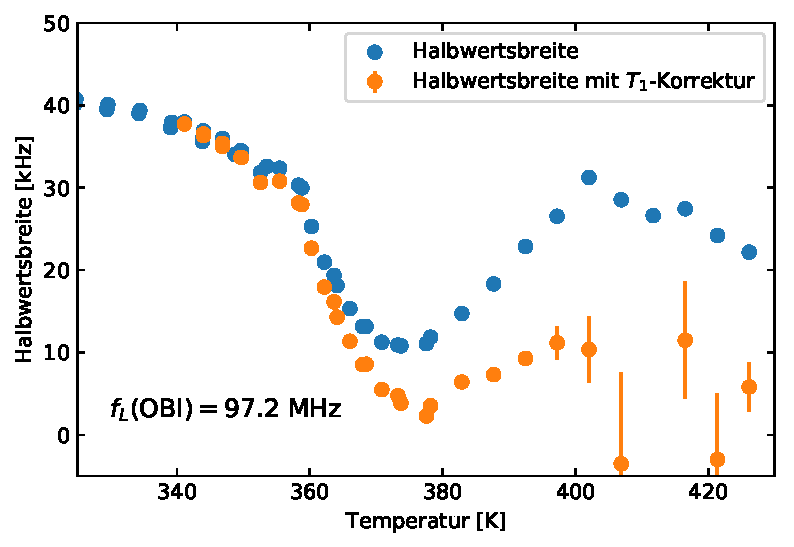
\includegraphics[width=.8\textwidth]{graphics/plot/fwhm_t1.pdf}
	\end{center}
	\caption{Halbwertsbreiten der OBI-Spektren in blau, mit der beschriebenen $T_1$-Korrektur in orange. Die gezeigten Unsicherheiten stammen aus den Unsicherheiten der $T_1$-Werte.} \label{fig:res:spek_fwhm_t1}
\end{figure}

Es ist zu erkennen, dass $T_1$ bei Temperaturen über $\SI{360}{\kelvin}$ einen großen Einfluss auf die Halbwertsbreite hat und die entsprechend angepassten Halbwertsbreiten deutlich geringere Werte aufweisen. Bei Temperaturen über $\SI{410}{\kelvin}$ können auch negative Halbwertsbreiten gefunden werden; diese sind aber aufgrund der hohen Schwankungen der $T_1$-Werte in diesem Temperaturbereich mit entsprechend hohen Unsicherheiten belegt. Eine präzisere Messung von $T_1$ würde eine Korrektur mit geringeren Unsicherheiten erlauben.




Es wurden die am OBI- und am Bruker-Spektrometer aufgenommenen Daten getrennt untersucht, da durch die unterschiedlichen Larmorfrequenzen abweichende Ergebnisse der theoretischen Kurven zu erwarten sind. Bei den Halbwertsbreiten wurde der $T_1$-Einfluss nach der beschriebenen Methode berücksichtigt.



Die aufgenommenen Spektren unterstützen eine biexponentielle Interpretation wie in \eqref{eqn:trans_relax} nur schwerlich, daher wurde lediglich der deutlich zu beobachtende Anteil des Zentralübergangs, $\Delta_c$ und $\omega_c^{(2)}$, für die entsprechenden FWHM- bzw. Schwer\-punkts-Da\-ten betrachtet. Für die $T_1$-Daten wird Formel \eqref{eqn:bpp} verwendet. Die Anpassung der Kurven wurde manuell durchgeführt.



Zunächst sollen die Daten des OBI-Spektrometers vergleichen werden. Bei den $T_1$-Werten soll erwähnt werden, dass die Werte bei hohen Temperaturen mit starken Unsicherheiten belegt sind (vgl. Abbildung \ref{fig:res:T_1}) -- entsprechende Indikatoren wurden hier für eine bessere Übersicht ausgelassen.

Für die Spektraldichte $J_\text{BPP}$ kann bei höheren Temperaturen, wie in Abbildung \ref{fig:res:theorie_j} zu sehen, mit dem Parameter $C_Q = \SI{3.6}{MHz}$ eine vergleichsweise gute Übereinstimmung für die Halbwertsbreiten und die Schwerpunkte erreicht werden. Zu tieferen Temperaturen gibt es jedoch gravierende Abweichungen. Für die stark ansteigenden Werte der Halbwertsbreite können anisotrope Effekte vermutet werden, deren Einfluss durch diese isotrope Theorie nicht abgedeckt wird und daher diesen Unterschied kreiert. Gründe für die Abweichungen der Schwerpunkte sind noch offen -- dieser Effekt wird jedoch gleichermaßen in experimentellen als auch simulierten Spektren beobachtet, was bedeutet, dass der Effekt vermutlich auf die von der Simulation berücksichtigten Wechselwirkungen eingeschränkt werden kann.
\begin{figure}
	\begin{center}
		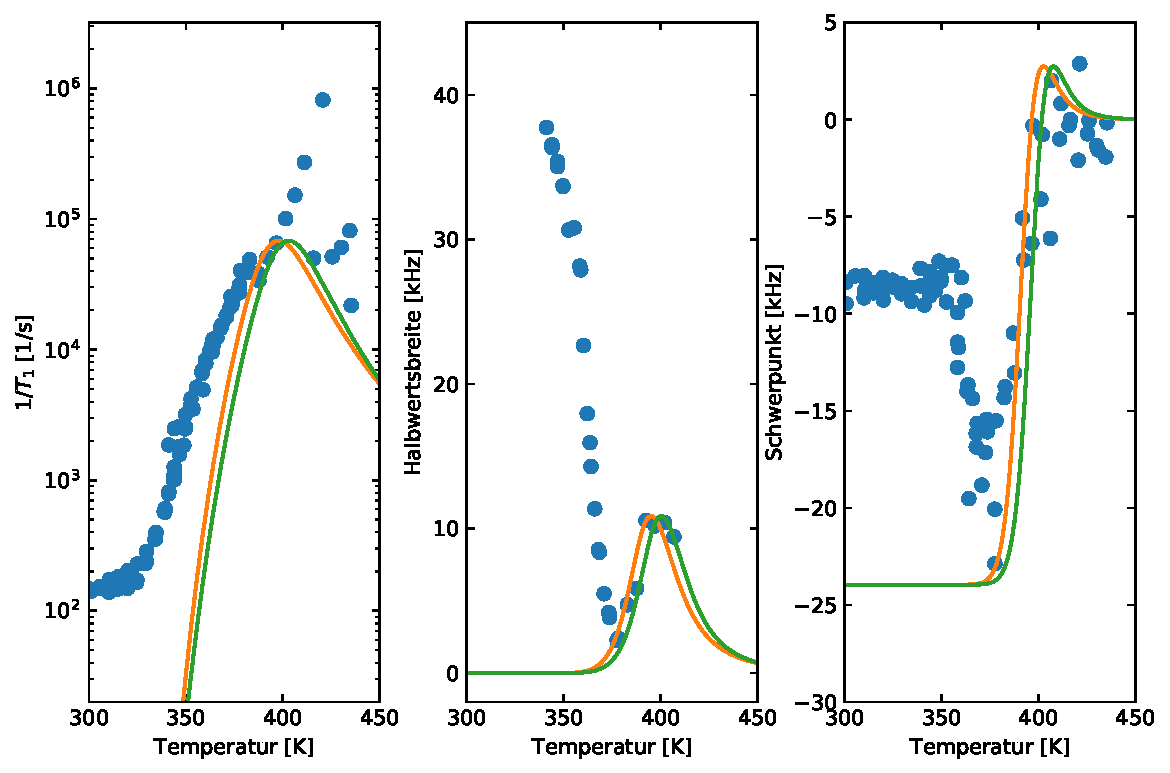
\includegraphics[width=.9\textwidth]{graphics/plot/OBI_J_02.pdf}
	\end{center}
	\caption{Vergleich von $T_1$, Halbwertsbreite und Schwerpunkt der OBI-Daten in blau. In orange die Theorie-Kurve mit Spektraldichte $J_\text{BPP}$ mit Parametern nach \cite{PIMENOV199793}, in grün mit Parametern nach \cite{crn_augsburg}.} \label{fig:res:theorie_j}
\end{figure}

Es kann eine grobe Vereinbarkeit der Theorie mit $T_1$-Werten im Maximum der Kurve erreicht werden, die Flanken unterscheiden sich jedoch deutlich. Da die Form der Theoriekurve mit der Spektraldichte $J_\text{BPP}$ unveränderlich ist, ist es schwerlich möglich, eine zufriedenstellende Übereinstimmung zu erreichen. Abhilfe schaffen könnten andere Spektraldichten -- dies soll im Folgenden untersucht werden.

Für die Spektraldichten $J_\text{CC}$ (Abbildung \ref{fig:res:theorie_j_cc}) und $J_\text{CD}$ (Abbildung \ref{fig:res:theorie_j_dc}) lagen die für die theoretische Berechnung der Schwerpunkte benötigten Imaginärteile $Q_\text{CC}$ und $Q_\text{CD}$ nicht vor, weswegen für diese auf die Spektraldichte $J_\text{BPP}$ zurückgegriffen wurde. Für die Schwerpunkte kann der Vergleich daher nur als grobe Idee verstanden werden.
\begin{figure}
	\begin{center}
		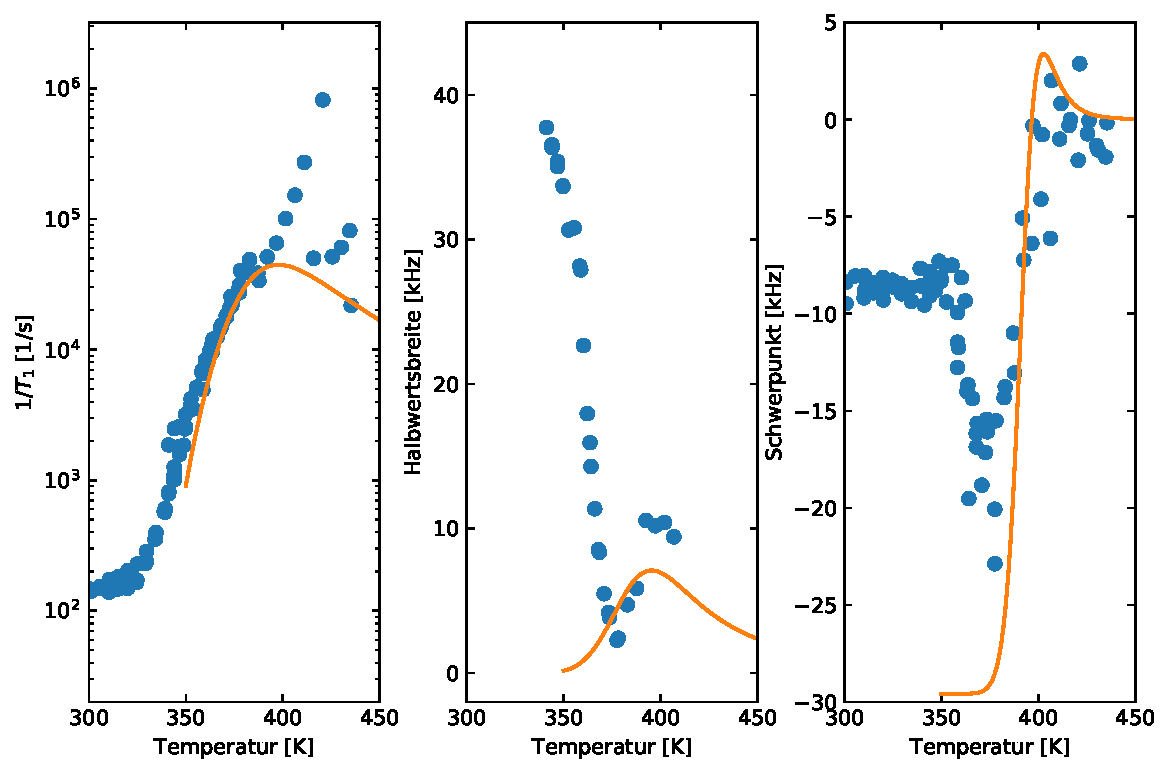
\includegraphics[width=.8\textwidth]{graphics/plot/OBI_J_cc_01.pdf}
	\end{center}
	\caption{Vergleich von $T_1$, Halbwertsbreite und Schwerpunkt der OBI-Daten in blau. In orange die Theoriekurve mit Spektraldichte $J_\text{CC}$ mit Parametern nach \cite{PIMENOV199793}.} \label{fig:res:theorie_j_cc}
\end{figure}
\begin{figure}
	\begin{center}
		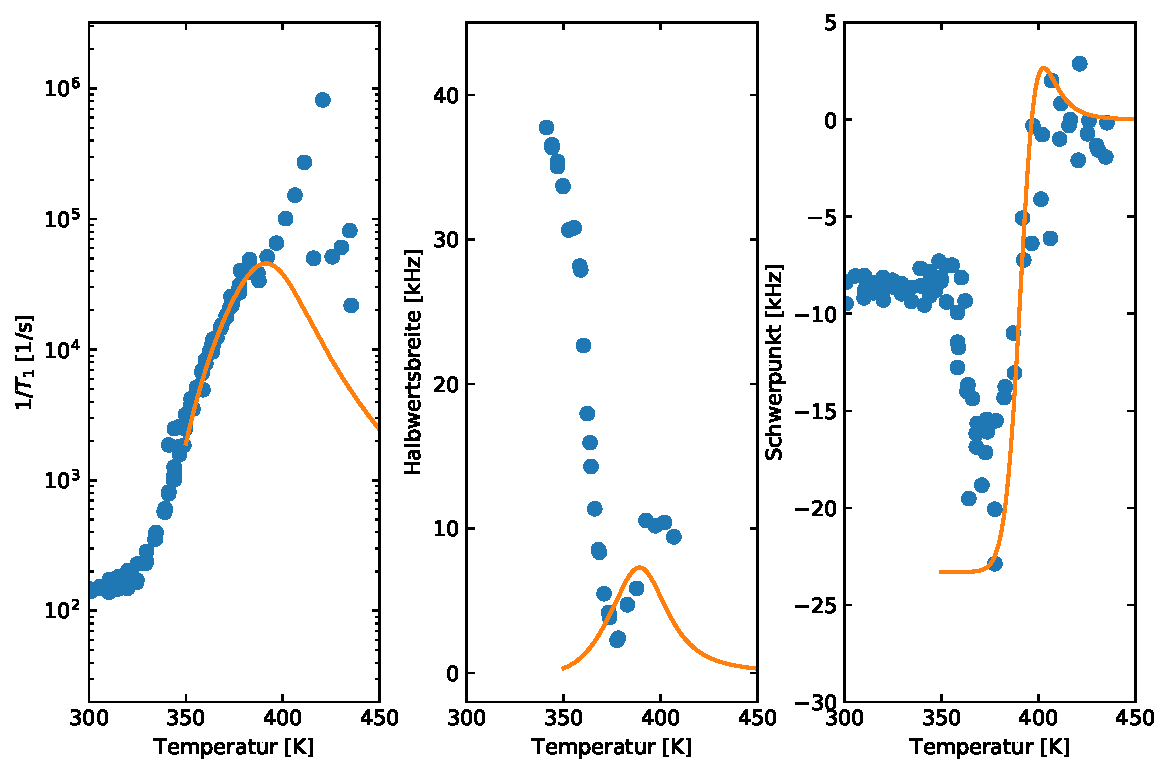
\includegraphics[width=.8\textwidth]{graphics/plot/OBI_J_dc_01.pdf}
	\end{center}
	\caption{Vergleich von $T_1$, Halbwertsbreite und Schwerpunkt der OBI-Daten in blau. In orange die Theorie-Kurve mit Spektraldichte $J_\text{CD}$ mit Parametern nach \cite{PIMENOV199793}.} \label{fig:res:theorie_j_dc}
\end{figure}

Für $J_\text{CC}$ und $J_\text{CD}$ können mit den Parametern $C_Q = \SI{4.0}{MHz}$ und $\alpha = \SI{0.6}{}$ bzw. $C_Q = \SI{3.6}{MHz}$ und $\gamma = \SI{0.46}{}$ gute Übereinstimmungen für $T_1$ beobachtet werden -- zumindest oberhalb einer Temperatur von etwa $\SI{350}{\kelvin}$. Für $J_\text{CD}$ scheint es zudem für Temperaturen über $\SI{400}{K}$ Abweichungen zu geben. Eine bessere Vereinbarkeit mit $T_1$-Werten kommt in beiden Fällen auf Kosten der vergleichsweise guten Übereinstimmungen für Halbwertsbreite und Schwerpunkt zustande, die mit $J_\text{BPP}$ erreicht werden konnten: Während für $J_\text{CC}$ die Schwerpunkte stark abweichen, ist dies bei $J_\text{CD}$ für die Halbwertsbreiten der Fall. Es bleibt festzuhalten, dass insgesamt eine gute Übereinstimmung mit der Theorie gezeigt werden konnte; es kann jedoch keine Spektraldichte besonders vorteilhaft hervorgehoben werden.

Für den Vergleich der Daten des Bruker-Spektrometers ist Ähnliches zu beobachten. Dabei fällt es hier aber schwerer, definitive Aussagen zu treffen, da der eingeschränkte Temperaturbereich nur einen bedingten Vergleich zulässt. Abbildung \ref{fig:res:theorie_bruker} zeigt die Daten zusammen mit Theoriekurven basierend auf der Spektraldichte $J_\text{BPP}$ mit dem Parameter $C_Q = \SI{3.45}{MHz}$. Dabei ist zu sehen, dass die Daten im gleichen Maße wie die OBI-Daten Übereinstimmungen und Unterschiede aufzeigen.
\begin{figure}
	\begin{center}
		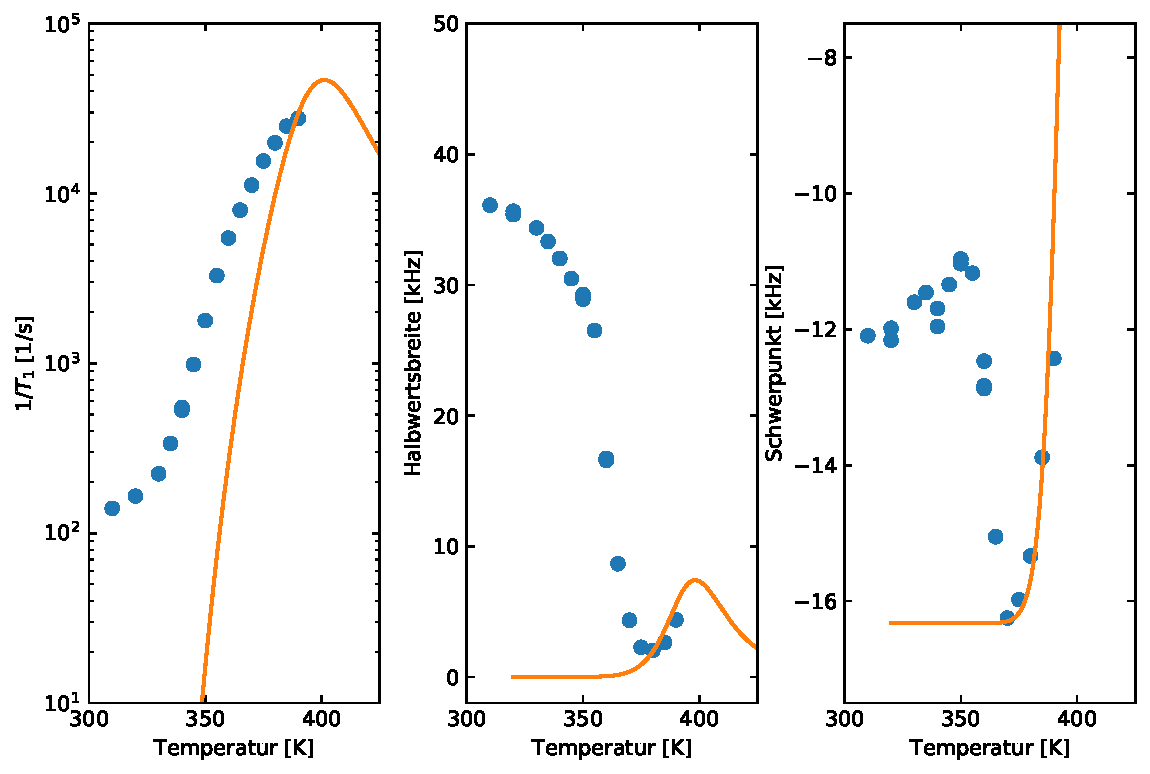
\includegraphics[width=.9\textwidth]{graphics/plot/Bruker_J_01.pdf}
	\end{center}
	\caption{Vergleich von $T_1$, Halbwertsbreite und Schwerpunkt der Bruker-Daten in blau. In orange die Theorie-Kurve mit Spektraldichte $J_\text{BPP}$ mit Parametern nach \cite{PIMENOV199793}.} \label{fig:res:theorie_bruker}
\end{figure}


